\section{Biohadoop}
\subsection{}
\begin{frame}
  \frametitle{Biohadoop basic concepts}
  \begin{itemize}
    \item Master-worker scheme:
    \begin{itemize}
      \item One \textbf{master} executes the main \textbf{algorithm} (e.g. GA)
      \item Parallel \textbf{workers} execute work intense computations (e.g. solution evaluation)
    \end{itemize}
    \vspace{0.5em}
    \begin{center}
      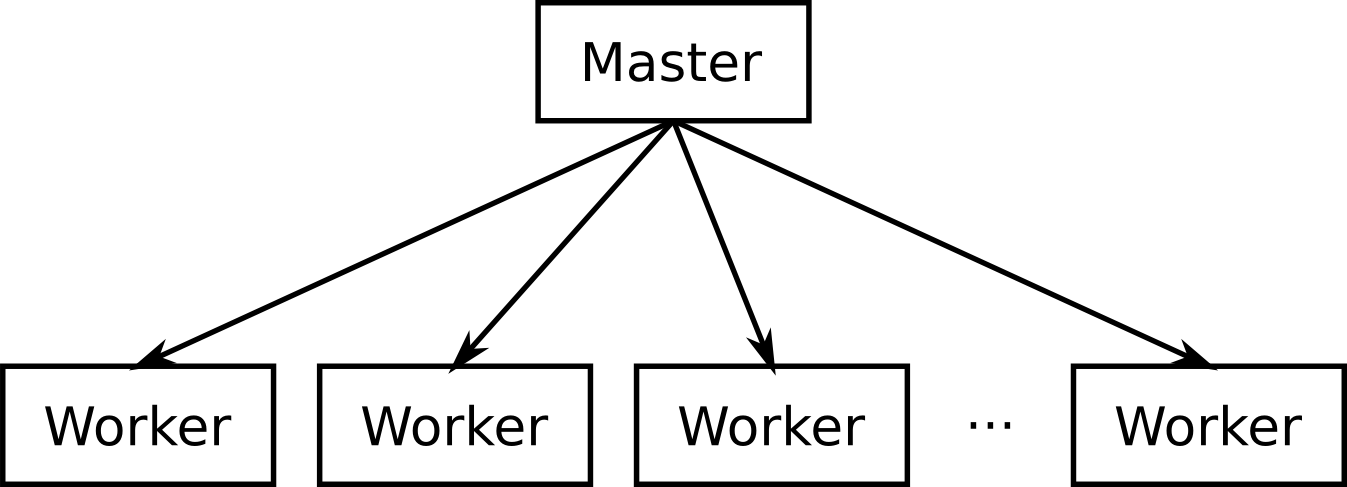
\includegraphics[width=50mm]{master-worker-simple.png}
    \end{center}
    \vspace{0.5em}
    \item Work items sent from master to workers are called \textbf{tasks}
    \item Workers compute \textbf{results} for tasks and return them to master
    \item Communication between master and workers is \textbf{asynchronous}
%     \item Java based
  \end{itemize}
\end{frame}
\begin{frame}
  \frametitle{System architecture}
  \begin{columns}
    \begin{column}{.7\textwidth}
      \begin{itemize}
        \item Algorithm
	\begin{itemize}
	  \item implements optimization problem and schedules tasks for workers
	\end{itemize}
	\item Task System
	\begin{itemize}
	  \item TaskBroker queues tasks an passes them to endpoint on request
	  \item Endpoint is the boundary of the master, workers communicate to endpoint
	  \item Worker(s) request tasks, compute solutions and return results
        \end{itemize}
      \end{itemize}
      \vspace{1em}
    \end{column}
    \begin{column}{.3\textwidth}
      \begin{center}
	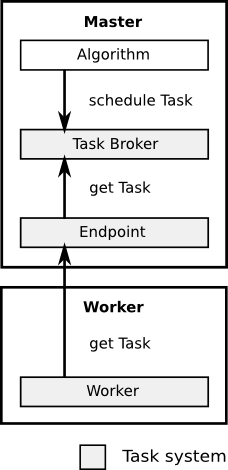
\includegraphics[width=30mm]{architecture-simple.png}
      \end{center}
    \end{column}
  \end{columns}
\end{frame}
\begin{frame}
  \frametitle{Biohadoop usage}
  Three steps to implement new algorithm:
  \begin{itemize}
    \item Implement \texttt{Algorithm} interface, executed on master - typically includes problems main loop
    \item Implement \texttt{Worker} interface, executed on workers - typically includes work intense computations
    \item Submit tasks from within the algorithm to the task system and wait (or not) for the results
  \end{itemize}
  \vspace{1em}
  Biohadoop takes care of the rest (Worker startup and shutdown, communication, failure detection)
\end{frame}

\begin{frame}
  \frametitle{Example: Genetic Algorithm}
  \begin{columns}
    \begin{column}{.7\textwidth}
      \begin{itemize}
	\item Generate initial population (master)
	\item Evaluate initial population (\textbf{worker})
	\item Main loop until termination (master):
	\begin{itemize}
	  \item Generate new solutions from current population (master)
	  \item Evaluate new solutions (\textbf{worker})
	  \item Select best overall solutions $\rightarrow$ current population for next iteration (master)
	\end{itemize}
	\item After termination, current population is solution to problem (master)
      \end{itemize}
    \end{column}
    \begin{column}{.3\textwidth}
      \begin{center}
	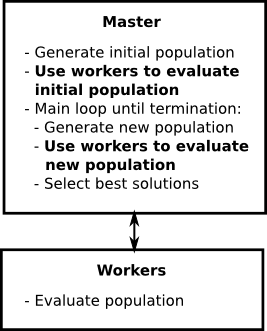
\includegraphics[width=30mm]{example-simple.png}
      \end{center}
    \end{column}
  \end{columns}
\end{frame}